\documentclass{article}
\usepackage[utf8]{inputenc}
\usepackage{amsmath}
\usepackage{amssymb}
\usepackage{mathtools}
\usepackage[fleqn]{nccmath}
\usepackage{enumitem}
\usepackage{indentfirst}
\usepackage{graphicx}
\usepackage{caption}
\usepackage{subcaption}
\usepackage{color} %red, green, blue, yellow, cyan, magenta, black, white
\usepackage[dvipsnames]{xcolor}
\usepackage{tikz,pgfplots,tikz-3dplot}
\usepackage{listings}
\usepackage{cancel}
\usepackage{braket}
\usepackage{esvect,esint}
\usepackage{float}
\usepackage{bm}
\usepackage{mdframed}
\usepackage{multirow}
\usepackage{multicol}
\usepackage{hyperref}
\hypersetup{
    colorlinks=true,
    filecolor=magenta,
    linkcolor=cyan,
    citecolor = red,
    pdftitle={Final Project Proposal}
    }
\usepackage{titling}
\usepackage{titlesec} % Section headings
\titleformat*{\section}{\large\bfseries}
\titleformat*{\subsection}{\normalsize\bfseries}
\titleformat*{\subsubsection}{\normalsize\bfseries}
\titlespacing{\section}{0pt}{10pt}{0pt}
\titlespacing{\subsection}{0pt}{10pt}{0pt}
\titlespacing{\subsubsection}{0pt}{10pt}{0pt}

\usepackage{geometry}
\geometry{
    a4paper,
    margin=1in, % Margin size, obviously.
    top = 1in,
    bottom = 0.5in,
}

\usepackage{fancyhdr}
\pagestyle{fancy}
\fancyhf{}
\lhead{Ethan Pham, Jo Mama}
\rhead{\thepage}

\usetikzlibrary{shapes, calc, arrows, arrows.meta, patterns, decorations.markings, decorations.pathmorphing, patterns.meta}

\def\centerarc[#1](#2)(#3:#4:#5)% Syntax: [draw options] (center) (initial angle:final angle:radius)
    { \draw[#1] ($(#2)+({#5*cos(#3)},{#5*sin(#3)})$) arc (#3:#4:#5); }

\usepackage{color} %red, green, blue, yellow, cyan, magenta, black, white
\graphicspath{ {./Images/} }

\definecolor{string}{RGB}{230, 219, 116}
\definecolor{comment}{RGB}{117, 113, 94}
\definecolor{normal}{RGB}{0,0,0}
\definecolor{identifier}{RGB}{166, 226, 46}

\lstset{
	language=python,                			% choose the language of the code
  	numbers=left,                   		% where to put the line-numbers
  	stepnumber=1,                   		% the step between two line-numbers.        
  	numbersep=5pt,                  		% how far the line-numbers are from the code
  	numberstyle=\tiny\color{black}\ttfamily,
  	showspaces=false,               		% show spaces adding particular underscores
  	showstringspaces=false,         		% underline spaces within strings
  	showtabs=false,                 		% show tabs within strings adding particular underscores
  	tabsize=4,                      		% sets default tabsize to 2 spaces
  	captionpos=b,                   		% sets the caption-position to bottom
  	breaklines=true,                		% sets automatic line breaking
  	title=\lstname,                 		% show the filename of files included with \lstinputlisting;
  	basicstyle=\color{normal}\ttfamily,					% sets font style for the code
  	keywordstyle=\color{magenta}\ttfamily,	% sets color for keywords
  	stringstyle=\color{string}\ttfamily,		% sets color for strings
  	commentstyle=\color{comment}\ttfamily,	% sets color for comments
  	emph={format_string, eff_ana_bf, permute, eff_ana_btr},
  	emphstyle=\color{identifier}\ttfamily
}

% Calculus Commands
\newcommand{\infint}{\int_{-\infty}^{\infty}}
\newcommand{\fd}[2]{\dfrac{\mathrm{d}^{#2}}{\mathrm{d}#1^{#2}}} % For full derivatives. \fd{variable}{number}
\newcommand{\ffd}[3]{\dfrac{\mathrm{d}^{#3}#1}{\mathrm{d}#2^{#3}}} % For full derivatives with function. \ffd{function}{variable}{number}
\newcommand{\pd}[2]{\dfrac{\partial^{#2}}{\partial #1^{#2}}} % For partial derivatives. \pd{variable}{number}
\newcommand{\fpd}[3]{\dfrac{\partial^{#3}#1}{\partial #2^{#3}}} % For partial derivatives with function. \fpd{function}{variable}{number}


% Number symbols
\newcommand{\R}{\mathbb{R}}
\newcommand{\N}{\mathbb{N}}
\newcommand{\Z}{\mathbb{Z}}
\newcommand{\Q}{\mathbb{Q}}

% Vector Commands
\renewcommand{\vv}[1]{\bm{\mathrm{#1}}}
\newcommand{\uvv}[1]{\hat{\bm{\mathrm{#1}}}}
\newcommand{\dvv}[1]{\dot{\bm{\mathrm{#1}}}}
\newcommand{\ddvv}[1]{\ddot{\bm{\mathrm{#1}}}}
\newcommand{\grad}{\bm{\mathrm{\nabla}}}
\newcommand{\abs}[1]{\left|#1\right|}

% Trig Commands
\newcommand{\arccot}{\operatorname{arccot}}
\newcommand{\csch}{\operatorname{csch}}
\newcommand{\sech}{\operatorname{sech}}

% QED
\newcommand{\qed}{\tag*{\(\square\)}}

% Typing Commands
\newcommand{\note}[1]{\color{red}#1\color{black}}


\pgfplotsset{compat=1.18}
\usepgfplotslibrary{colorbrewer}

\begin{document}
\section*{Graviational Lensing for a Schwarzschild Black Hole using Backwards Ray Tracing}
	General relativity says that matter tells space how to bend, and space tells matter how to move. Assuming a cosmological constant of zero, this relation is governed by the Einstein field equations:
	\begin{align}
		R_{\mu\nu}-\frac{1}{2}R=8\pi G T_{\mu\nu}
	\end{align}
	The Schwarzschild solution is the simplest case; a completely stationary mass centered at the origin, whose metric (using \(-,+,+,+\)) in spherical coordinates is well known to be
	\begin{align}
		\mathrm{d}s^{2}=-\left(1-\frac{r_{s}}{r}\right)\mathrm{d}t^{2}+\left(1-\frac{r_{s}}{r}\right)^{-1}\mathrm{d}r^{2}+r^{2}\mathrm{d}\theta^{2}+r^{2}\sin^{2}\theta\mathrm{d}\phi^{2}
	\end{align}
	The spherical symmetry of the problem allows us to calculate the geodesics in a plane (\(\theta=\pi/2\)). We can write a pair of differential equations for \(r\) and \(\phi\) in terms of the conserved quantities energy \(E\) and angular momentum \(L\):
	\begin{align} \label{eq:eom}
		\begin{aligned}
			\dot{\phi}&=\frac{L}{r^{2}}, & \ddot{r}&=-\frac{R_{s}}{2r^{2}}\left(\frac{L^{2}}{r^{2}}+\epsilon\right)+\frac{L^{2}}{r^{3}}\left(1-\frac{R_{s}}{r}\right)
		\end{aligned}
	\end{align}
	Where the quantity \(\epsilon=0\) since light travels on null geodesics. These equations can be solved numerically on a computer to generate the path that light takes in the presence of a Schwarzschild black hole. 
	
	Looking towards a background galaxy with a black hole in front of it will caused the resulting image for the observer to be distorted, as the mass of the black hole bends light around it in such a way that it is possible to see two (or more) images of the same light source. This effect is normally done computationally using a thin lens approximation to derive formulas for the angle of deflection which can then be used to distort an image (which is used as the background galaxy) as if it emitted parallel light rays towards black hole.
	
	The lensing effect should be reproducible using ray tracing methods as well. By considering each pixel of an image (as the background galaxy) and casting rays out toward the black hole and hit some target plane (observer) to map the pixels of the image their corresponding locations in the target plane where the trajectories can be obtained using the light geodesics discussed above.
	
\subsection*{Approach}
Figuring out the photon trajectories comes down to integrating the equations of motion \ref{eq:eom} with the either the Richardson extrapolation \cite{Richardson extrapolation} (along with the usual Runge-Kutta 4 method) or the Runge-Kutta-Fehlberg method (also known as RK45) for dynamic time stepping and increased rate of convergence, whichever ends up working. The energy \(E\) and angular momentum \(L\) are both determined by initial conditions. 

The ray tracing method used will be backwards ray tracing. The reasoning is as follows: ray tracing involves casting out several rays, then letting them hit surfaces, bounce around, and so on until they reach the position of some observer. This process is described as forward ray tracing, and is generally very inefficient. This is because most of the rays cast from the light source will never actually reach the camera, perhaps being reflected to somewhere far off or obstructed by some black body. In turn this uses a lot of unnecessary computation and so to remedy this, we take rays cast from the observer and track what they hit instead. These rays are guaranteed to have ``hit" the camera, since they started there to begin with, but more formally: this solution works because running time backwards (\(t\to -t\)) will give the effect of reversing the direction the ray took to get to the object. In other words, it makes it look like the object emitted the rays which then bounced around and hit the camera.

\begin{figure}[H]
	\centering
	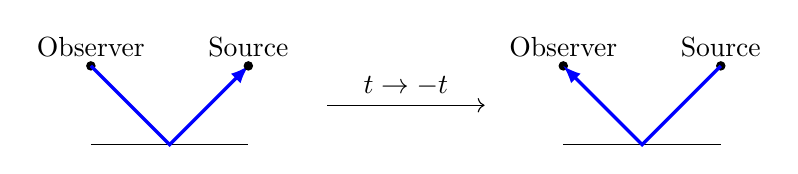
\begin{tikzpicture}
		\draw[-](-4,0)--(-2,0);
		\filldraw[black] (-4,1) circle (1.5pt) node[above]{Observer};
		\draw[-latex,very thick, blue](-4,1)--(-3,0)--(-2,1);
		\filldraw[black] (-2,1) circle (1.5pt) node[above]{Source};
		\draw[->](-1,0.5)--(1,0.5)node[midway,above]{$t\to -t$};
		\draw[-](4,0)--(2,0);
		\filldraw[black] (4,1) circle (1.5pt) node[above]{Source};
		\filldraw[black] (2,1) circle (1.5pt) node[above]{Observer};
		\draw[-latex,very thick, blue](4,1)--(3,0)--(2,1);
	\end{tikzpicture}
	\caption{Backward Ray Tracing}
\end{figure}

In particular, time reversal works for light geodesics, as the they are (with valid initial conditions) unique for the Schwarzschild metric. We will make an image by sending out rays with initial conditions backwards from the start plane toward the black hole, let it do whatever it does and eventually one of four outcomes can occur. 
\begin{enumerate}
	\item It enters the black hole, which we set that pixel to black and terminate the calculation, since once inside the black hole it can never leave.
	\item It hits the image, in which case we take the color of the pixel and map it back to where the ray started.
	\item It shoots off to infinity (out of bounds) in which case we also set to black. (Note: While debugging, we may set the pixel to a different color depending on whether it enters the black hole or goes out of bounds.)
	\item It happens to be a special trajectory (or near one) whose solutions end up orbiting the black hole indefinitely, or for a long period of time, which can be solved by enforcing a limit to the number of iterations in the integrator.
\end{enumerate}
In theory, this should allow us to get the same distortion effects that are obtained using lensing equations and angles of deflection (which seems to be the most common way to do this). 

\subsection*{Objectives}
\begin{enumerate}
	\item Simulate and render a 3D trajectory for a single photon.
	\item Check simulation by using known solutions (i.e. ICs where light orbits the black hole are known, so setting those in the simulation should match).
	\item Generate an image displaying the lensing effect using a ``background galaxy" (which will probably be an image off of Google). Or if this is too computationally expensive, use a lower resolution image. Using a checkerboard pattern as the image will allow us to clearly see the lensing effect. 
	\item Compare the results with other (physically correct) lensing simulations (like this one from NASA \cite{NASA}, Harvard \cite{Harvard}, or some of the examples on Wikipedia \cite{Wikipedia}) and see how well it matches.
\end{enumerate}

\subsection*{Stretch Goals}
\begin{enumerate}
	\item Translate or tilt the image it at an angle to simulate changing the perspective of the lensing and make a short video displaying the lensing effect.
	\item Lens with a different metric (Kerr, Kerr-Newmann, etc.) for a rotating or charged (or a combination of the two) black hole. 
\end{enumerate}

\subsection*{Approval}
\begin{itemize}
	\item Ethan approves of this proposal!
	\item Jo approves of this proposal!
\end{itemize}

\newpage
\begin{thebibliography}{5}
	\bibitem{Richardson extrapolation}
	Joel Feldman (2000) \url{https://personal.math.ubc.ca/~feldman/m256/richard.pdf}
	
	\bibitem{RK45}
	Gurevich, Svetlana (2017) \url{https://www.uni-muenster.de/imperia/md/content/physik_tp/lectures/ss2017/numerische_Methoden_fuer_komplexe_Systeme_II/rkm-1.pdf}
	
	\bibitem{NASA}
	STScI/Frank Summers (2003) \url{https://www.youtube.com/watch?v=k6JHryhlNVk}
	
	\bibitem{Harvard}
	\url{https://lweb.cfa.harvard.edu/~bmcleod/castlepress.html}
	
	\bibitem{Wikipedia}
	\url{https://en.wikipedia.org/wiki/Gravitational_lens}
	
	
\end{thebibliography}
	
	
	
	
\end{document}